\section{Sesión 1}

\subsection{Transformaciones en el plano}

\begin{definicion}
	\begin{enumerate}
		\item 	Una transformación en el plano es una función que le asigna a cada punto en el plano otro punto en el plano al cuál llamaremos imagen. 
		\item Una transformación a una figura en el plano obtenemos una nueva figura que llamaremos la transformada.
	\end{enumerate}
\end{definicion}

\subsubsection{Clases}

\begin{enumerate}
	\item \textbf{Isométricas}: transformaciones que conservan \textbf{la forma, las longitudes, las áreas y ángulos(en magnitud) de una figura.}
	\begin{enumerate}
		\item \textbf{Traslación}: Sea $A$ un punto en el plano y $\vec{v}$ un vector, una traslación en el plano se dará cuando cada punto de la figura se mueva en la dirección de $\vec{v}$.
		 \begin{center}
			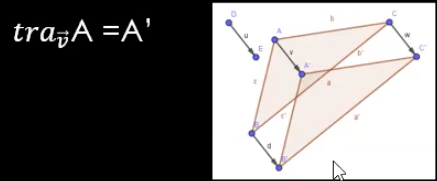
\includegraphics[scale=0.5]{images/Sesion1/1}
		\end{center} 
	\item \textbf{Reflexión o Simetría:} Existen dos clases de reflexiones. 
	\begin{enumerate}
		\item \textbf{Puntual o central:} Cuando reflejamos una figura respecto a un punto. [$Ref(0)$]  \begin{center}
				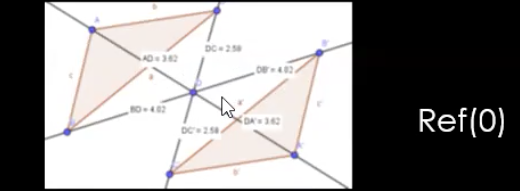
\includegraphics[scale=0.5]{images/Sesion1/2.png}
		\end{center}
		\item \textbf{Axial:} Reflejamos la figura respecto a una recta, llamada eje de reflexión. [$Ref(I)$]  \begin{center}
		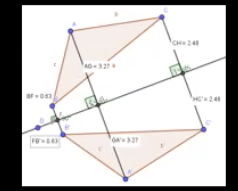
\includegraphics[scale=0.5]{images/Sesion1/3.png}
	\end{center}
	\end{enumerate}
\item \textbf{Rotación}: Es una transformación que cambia la dirección de una figura, en este caso se tiene un punto fijo 0 y un ángulo constante (positivo o negativo). La distancia del punto al 0 es constante. 
 \begin{center}
	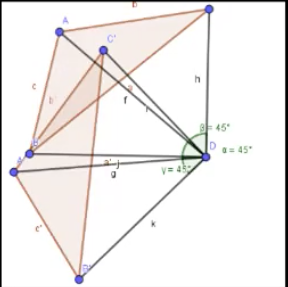
\includegraphics[scale=0.5]{images/Sesion1/4.png}
\end{center}
	\end{enumerate}
	\item \textbf{No isométricas}: son aquellas transformaciones que alteran la forma y dimensión de la figura. 
	\begin{enumerate}
		\item \textbf{Homotecia}: es una transformación en la que se obtiene una figura a escala de la original, se necesita un punto fijo 0 y una constante de proporcionalidad $k$. 
		\begin{enumerate}
			\item Cambia longitudes y áreas pero conserva ángulos.
			\item Si $k>0$ conserva la dirección. 
			\item Si $k<0$ se obtiene la dirección opuesta.
		\end{enumerate}
	 \begin{center}
		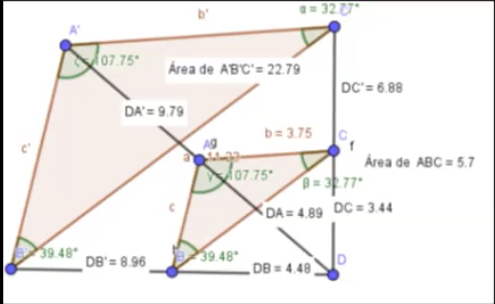
\includegraphics[scale=0.5]{images/Sesion1/5.png}
	\end{center}
	\end{enumerate}
\end{enumerate}

\subsubsection{Notación}

\textbf{Isométricas}
\begin{enumerate}
	\item Traslación: $\operatorname{Tra}\overrightarrow{AB}$.
	\item Reflexión: 
	\begin{enumerate}
		\item $\operatorname{Ref}(0)$. 
		\item $\operatorname{Ref}(l)$. 
	\end{enumerate}
\item Rotación: $\operatorname{Rot}(A,\theta)$.
\item Homotecia:  $\operatorname{Hom}(A,k)$.
\end{enumerate}

\begin{ejemplo}
	$$\triangle \operatorname{ABC}:\quad \operatorname{Hom}(A'', 2)\circ \operatorname{rot}(0,30^{\circ})\circ \operatorname{Rel}(B) $$
\end{ejemplo}
